\section*{Proximity Based Real Time Alert System Using Monocular Depth Estimation Through RT MonoDepth And YOLO11}

\textbf{Farooqui U Rizwan\textsuperscript{1}, Ashwani Kumar Mishra\textsuperscript{2}, Asad Waqar Malik\textsuperscript{3}, and Abid Hassan\textsuperscript{4}}

\vspace{0.5cm}
\footnotesize{
\noindent
\textsuperscript{1}Department of Building Construction Science, Mississippi State University, Starkville, USA\\
\textsuperscript{2}Department of Computer Science \& Engineering, Mississippi State University, Starkville, USA\\
\textsuperscript{3}NSPARC, Mississippi State University, Starkville, USA\\
\textsuperscript{4}Department of Industrial \& Systems Engineering, Mississippi State University, Starkville, USA
}
\vspace{0.5cm}

\section*{Abstract}
[cite_start]"Struck-by-equipment" incidents are a leading cause of fatalities in the construction industry, highlighting a critical need for proactive safety systems[cite: 8]. [cite_start]While computer vision technologies like object detection and monocular depth estimation (MDE) have advanced independently, a significant barrier to their practical application in safety monitoring has been MDE's inherent scale ambiguity, which prevents direct metric distance measurement[cite: 9]. [cite_start]This paper introduces a unified, real-time framework that synergistically integrates state-of-the-art object detection (YOLOv11) and MDE (RT-MonoDepth) to overcome this limitation[cite: 10]. [cite_start]Our primary contribution is a novel automatic geometric calibration method that resolves scale ambiguity by using detected personnel as an anthropometric reference, enabling the system to produce precise, object-specific distance measurements in meters from a single uncalibrated camera[cite: 11]. [cite_start]By executing these models concurrently in a multi-threaded pipeline, the system transforms standard 2D video into an actionable source of 3D spatial intelligence, reconstructing the scene to calculate true Euclidean distances between workers and machinery[cite: 12]. [cite_start]The framework's efficient architecture was validated on construction site footage, demonstrating robust real-time performance (25.4 FPS at 39.3 ms latency) that confirms its suitability for deployment on resource-constrained, edge-computing platforms like the NVIDIA Jetson Nano[cite: 13]. [cite_start]The system successfully identified proximity hazards and quantitatively logged events where safety zones were breached, proving its efficacy as a practical monitoring tool[cite: 14]. [cite_start]This framework presents a cost-effective and deployable alternative to expensive hardware like LiDAR, offering a viable path toward reducing injuries and fatalities by turning simple video feeds into an advanced situational awareness system[cite: 15].

\vspace{0.3cm}
\noindent \textbf{Keywords:} Metric Monocular Depth Estimation, Construction Safety, YOLOv11, RT MonoDepth, Realtime systems, Artificial Intelligence, Machine Learning.

\section{Introduction}
[cite_start]The construction industry is one of the most dangerous sectors worldwide, with "struck-by-equipment" incidents being a leading cause of fatalities (Pan \& Zhang, 2021)[cite: 19]. [cite_start]To mitigate these risks, artificial intelligence and computer vision systems are increasingly being explored to provide proactive risk management and turn reactive safety protocols into preventative ones[cite: 20]. [cite_start]Two key technologies have emerged as foundational for this goal: object detection and depth estimation[cite: 21].

[cite_start]Advances in object detection, particularly with models like YOLO, have enabled robust, real-time identification and segmentation of critical agents like workers and machinery on complex construction sites (He et al., 2024; Pan \& Zhang, 2021)[cite: 22]. [cite_start]Concurrently, monocular depth estimation (MDE) has matured into a cost-effective alternative to expensive hardware like LiDAR, with modern lightweight networks achieving real-time performance on embedded systems (Feng et al., 2024; Masoumian et al., 2022)[cite: 23]. [cite_start]These models can generate dense depth maps from a single, inexpensive camera, providing crucial spatial information about a scene[cite: 24].

[cite_start]Despite these parallel advancements, a critical gap remains between the capabilities of individual models and the needs of a practical, deployable safety system[cite: 25]. [cite_start]Object detection answers \textit{what} an object is but provides no spatial depth[cite: 26]. [cite_start]MDE, conversely, provides spatial data but lacks semantic understanding and is fundamentally limited by an inherent scale ambiguity—its output is a relative depth map without real-world units, rendering it unusable for metric distance measurement (Zhang et al., 2025; Shen et al., 2023)[cite: 27]. [cite_start]This ambiguity has been a primary barrier preventing the widespread adoption of MDE for safety-critical applications[cite: 28].

[cite_start]While the potential of fusing these two technologies has been explored, for example by Yu \& Choi (2021) in their YOLO MDE framework, the challenge of resolving scale ambiguity in a practical, on-the-fly manner persists[cite: 29]. [cite_start]Many approaches still fall short of providing a truly deployable solution that can operate with uncalibrated, monocular cameras in dynamic environments[cite: 30].

[cite_start]This paper bridges this gap by introducing a unified framework that synergistically integrates state-of-the-art object detection (YOLOv11) and MDE (RT-MonoDepth) into a single, end-to-end system[cite: 31]. [cite_start]Our primary contribution is a novel automatic geometric calibration method that resolves scale ambiguity by using detected personnel as an anthropometric reference, enabling the system to produce precise, object-specific distance measurements in meters from a single uncalibrated camera[cite: 32]. [cite_start]By running these models concurrently in a multi-threaded pipeline, our system transforms standard 2D video into an actionable source of 3D spatial intelligence, creating a deployable safety tool that can proactively identify and log proximity hazards in real-time on construction sites[cite: 33].

\section{Methods}

\subsection{System Architecture and Real-Time Processing Pipeline}
[cite_start]The methodology is built upon the RT-MonoDepth framework, a comprehensive real-time computational pipeline engineered specifically for construction site monitoring applications through the synergistic integration of monocular depth estimation and semantic object detection algorithms[cite: 37]. [cite_start]The system architecture processes continuous video streams through a sophisticated multi-modal input acquisition pipeline, generating dense disparity maps augmented with object-specific semantic metadata and spatial relationships without requiring stereo-pair camera configurations or active depth sensing hardware[cite: 38].

\begin{figure}[htbp]
    \centering
    \includegraphics[width=\linewidth]{figure1.png}
    \caption{RT-MonoDepth Parallel Processing Architecture. This figure demonstrates the concurrent execution paradigm that enables real-time performance characteristics.}
    \label{fig:architecture}
\end{figure}

[cite_start]Figure \ref{fig:architecture} presents the parallel processing architecture[cite: 39]. [cite_start]The core architectural foundation employs the RT-MonoDepth neural network, utilizing a sophisticated ResNet encoder-decoder topology with skip connections to infer metric depth information from monocular RGB images (Feng et al. 2023)[cite: 40]. [cite_start]The system integrates platform-specific hardware acceleration libraries, including MLX optimization for Apple Silicon architectures and CUDA acceleration for NVIDIA embedded platforms such as Jetson series processors, achieving sustained processing throughputs exceeding 30 FPS with end-to-end computational latency under 50ms[cite: 41].

\subsection{Multi-threaded Parallel Processing Architecture and Real-time Optimization}
[cite_start]The system's real-time performance characteristics are achieved through a sophisticated parallel processing architecture (Figure \ref{fig:architecture}), orchestrated by the \texttt{realtime\_depth\_video.py} script managing data ingestion from heterogeneous input modalities including live webcam feeds, pre-recorded video sequences, and real-time streaming protocols[cite: 43]. [cite_start]The architecture implements a producer-consumer threading paradigm with minimalist queue-based buffering mechanisms designed to mitigate computational latency and ensure responsive real-time operation under varying processing loads[cite: 44].

[cite_start]The threading architecture utilizes dual-queue synchronization primitives implemented through Python's \texttt{threading.Queue} interface: a primary \texttt{frame\_queue} and bidirectional \texttt{result\_queue}, each configured with maximum buffer capacity of unity (\texttt{maxsize=1})[cite: 45]. [cite_start]This configuration implements an intelligent automatic frame-dropping mechanism that prevents accumulation of temporal artifacts in memory buffers while facilitating lock-free concurrent execution when processing pipeline latency exceeds frame acquisition intervals[cite: 46]. [cite_start]The zero-copy memory management approach minimizes data transfer overhead between processing threads[cite: 47].

[cite_start]A dedicated \texttt{DepthFrameProcessor} thread, implemented as a subclass of \texttt{threading.Thread}, orchestrates concurrent execution of the primary machine learning inference engines[cite: 48]. [cite_start]This specialized thread manages simultaneous RT-MonoDepth depth estimation and YOLOv11 object detection inference operations on identical input frame tensors, enabling true parallel processing without blocking the main visualization and user interface loops[cite: 49]. [cite_start]The parallelized architectural design isolates distinct computational tasks including frame acquisition, ML model inference, sensor fusion processing, and output rendering, thereby preventing blocking I/O operations while maintaining fluid user interface responsiveness and system stability[cite: 50].

\subsection{Monocular Depth Estimation Neural Architecture and Implementation}
[cite_start]The depth estimation module implements RT-MonoDepth, a neural network architecture derived from the Monodepth2 framework with substantial architectural optimizations for high-throughput real-time inference applications (Feng et al. 2023)[cite: 53]. [cite_start]The system incorporates dynamic model selection capabilities, automatically detecting and deploying either the full-scale \texttt{DepthDecoder} or computationally optimized compact \texttt{DepthDecoderS} model variants based on weight file path analysis and system resource availability[cite: 54].

\begin{figure}[htbp]
    \centering
    \includegraphics[width=\linewidth]{figure2.png}
    \caption{RT-MonoDepth Data Transformation Flow. The diagram illustrates the sequential processing stages from raw RGB input through disparity estimation to final 3D world coordinate generation.}
    \label{fig:dataflow}
\end{figure}

[cite_start]As illustrated in the data transformation flow (Figure \ref{fig:dataflow}), the neural network processes raw RGB input tensors with standardized spatial dimensions of $640 \times 480 \times 3$ pixels through a comprehensive preprocessing pipeline including aspect ratio preservation, color space normalization, and tensor standardization[cite: 55]. [cite_start]The architecture comprises two primary computational components integrated through residual connections[cite: 56]. [cite_start]The encoder network utilizes hierarchical convolutional feature extraction layers implementing multi-scale spatial representation learning[cite: 57]. [cite_start]The ResNet backbone architecture captures contextual semantic information through progressively deeper feature maps with increasing receptive field coverage[cite: 58]. [cite_start]Skip connections preserve fine-grained spatial details while enabling gradient flow optimization during training phases[cite: 59].

[cite_start]The decoder network implements transposed convolutional upsampling operations with bilinear interpolation to generate high-resolution disparity maps from compressed feature representations[cite: 60]. [cite_start]Multi-scale output generation enables supervision at multiple resolution levels, enhancing depth estimation accuracy across varying object scales and distances[cite: 61]. [cite_start]The network outputs normalized disparity values ($\text{disp} \in [0,1]$) representing inverse depth relationships[cite: 62].

The conversion to metric depth measurements utilizes the \texttt{disp\_to\_depth} transformation function implementing the following mathematical formulation:

\begin{equation}
    \text{min\_disp} = 1 / \text{max\_depth}
\end{equation}
\begin{equation}
    \text{max\_disp} = 1 / \text{min\_depth}
\end{equation}
\begin{equation}
    \text{scaled\_disp} = \text{min\_disp} + (\text{max\_disp} - \text{min\_disp}) \times \text{disp}
\end{equation}
\begin{equation}
    \text{Depth} = 1 / \text{scaled\_disp}
\end{equation}

[cite_start]This formulation maintains the inverse relationship between disparity and depth while providing bounded output ranges suitable for subsequent processing stages[cite: 68]. [cite_start]The depth range parameters ($\text{min\_depth} = 0.1\text{m}$, $\text{max\_depth} = 100\text{m}$) are configured based on typical construction site monitoring requirements and camera positioning constraints[cite: 69].

\subsection{Integrated Object Detection and Semantic Scene Understanding}
[cite_start]For comprehensive semantic scene understanding and object recognition capabilities, the framework integrates YOLOv11 object detection implementing an anchor-free detection paradigm with Non-Maximum Suppression (NMS) post-processing algorithms[cite: 71]. [cite_start]The implementation supports both standard pre-trained model weights and custom-trained models specifically optimized for construction environment object taxonomy, including personnel classification, heavy machinery identification, and vehicular detection across diverse construction site scenarios[cite: 72].

[cite_start]The object detection pipeline executes in true parallel fashion with depth estimation processes, as demonstrated in Figure \ref{fig:architecture}, processing identical RGB frame tensors through separate convolutional backbone feature extraction networks[cite: 73]. [cite_start]This concurrent processing approach minimizes computational overhead while maximizing information extraction from each input frame[cite: 74]. [cite_start]The YOLOv11 architecture utilizes efficient backbone networks with Feature Pyramid Network (FPN) integration for multi-scale object detection across varying size categories[cite: 75].

[cite_start]Advanced class-specific confidence thresholding mechanisms are employed with adaptive parameters optimized for construction site monitoring applications: $\tau=0.25$ for personnel detection (prioritizing safety-critical human presence detection) and $\tau=0.35$ for machinery and vehicular classes (reducing false positive detections from complex construction equipment)[cite: 76]. [cite_start]These threshold values were empirically determined through extensive validation on construction site datasets to balance detection sensitivity with precision requirements[cite: 77].

[cite_start]Post-processing heuristics implement sophisticated geometric constraint optimization for dynamic vehicle-to-machinery reclassification procedures[cite: 78]. [cite_start]The classification refinement algorithm analyzes bounding box aspect ratios, relative frame coverage metrics, and geometric shape characteristics to contextually distinguish between standard vehicles and heavy construction equipment, ensuring accurate semantic labeling appropriate for construction site safety analysis scenarios[cite: 79]. The object detection system implements a hierarchical classification taxonomy specifically designed for construction environments:
\begin{itemize}
    [cite_start]\item \textbf{Personnel Class:} Workers, safety personnel, supervisors, and visitors [cite: 81]
    [cite_start]\item \textbf{Heavy Machinery Class:} Excavators, bulldozers, cranes, loaders, and specialized construction equipment [cite: 82]
    [cite_start]\item \textbf{Vehicle Class:} Trucks, vans, service vehicles, and material transport vehicles [cite: 83]
    [cite_start]\item \textbf{Safety Equipment:} Hard hats, safety vests, and protective gear (filtered from primary detection outputs) [cite: 84]
\end{itemize}
[cite_start]This taxonomy enables targeted safety monitoring and proximity analysis between different object categories, supporting comprehensive construction site management applications[cite: 85].

\subsection{Scale Calibration Methodology}
[cite_start]The primary calibration methodology implements automatic geometric calibration via the \texttt{auto\_calibrate\_scale} function, leveraging anthropometric scale estimation principles using detected personnel as reference objects with predefined real-world dimensional parameters[cite: 87]. [cite_start]The algorithm assumes an average human height of 1.7 meters, representing statistical anthropometric data for adult populations in construction environments[cite: 88]. Utilizing the pinhole camera model geometric relationships, metric depth $Z$ to detected objects is estimated through the fundamental relationship:

\begin{equation}
    Z = (f_y \cdot \text{ObjectHeight}_{\text{real}}) / \text{ObjectHeight}_{\text{pixels}}
\end{equation}

[cite_start]Where $f_y$ is the camera's focal length in the y-axis (in pixels), $\text{ObjectHeight}_{\text{real}}$ corresponds to the assumed real-world object height (1.7m for human subjects), and $\text{ObjectHeight}_{\text{pixels}}$ represents the detected bounding box height measured in pixel coordinates within the image plane[cite: 91]. [cite_start]Starting here, $Z$ will be referred as calibrated depth value[cite: 92].

[cite_start]Scale factor candidates are computed through comprehensive ratio analysis comparing geometrically derived depth estimates with network-predicted unscaled depth values at corresponding spatial locations[cite: 93]. The system implements robust statistical filtering to eliminate outlier measurements caused by detection errors or geometric constraint violations. Temporal smoothing via Exponential Moving Average (EMA) filtering provides robust scale factor adaptation with configurable smoothing parameters:

\begin{equation}
    \text{scale\_factor}(t) = \alpha \times \text{scale\_factor}(t-1) + (1-\alpha) \times \text{scale\_candidate}(t)
\end{equation}

[cite_start]The smoothing coefficient $\alpha=0.1$ was empirically determined to balance responsiveness to scale changes while maintaining stability against measurement noise[cite: 96]. [cite_start]This temporal filtering approach ensures consistent depth calibration across video sequences while accommodating gradual changes in scene geometry or camera positioning[cite: 97].

[cite_start]Alternative manual calibration mechanisms permit operator adjustment through interactive \texttt{user\_scale} parameters enabling real-time scale factor modification for precise real-world distance matching[cite: 98]. [cite_start]The interactive calibration interface supports keyboard-based scale adjustment ('+'/'-' keys) allowing operators to fine-tune depth measurements against known reference distances within the construction site environment[cite: 99]. [cite_start]This dual-calibration approach ensures system adaptability across diverse deployment scenarios and camera configurations[cite: 100].

\subsection{3D Coordinate Transformation and Spatial Reconstruction}
[cite_start]Upon obtaining calibrated metric depth maps through the scale resolution procedures detailed in Section 2.5, the system performs comprehensive 3D geometric reconstruction to project each 2D pixel coordinate ($u, v$) into the corresponding 3D world coordinate system ($X, Y, Z$)[cite: 102]. [cite_start]This spatial transformation enables quantitative distance measurements and proximity analysis between detected objects within the reconstructed scene space[cite: 103].

[cite_start]The 3D reconstruction process utilizes the pinhole camera model with camera intrinsic parameters ($f_x, f_y, c_x, c_y$) representing focal lengths and principal point coordinates respectively[cite: 104]. [cite_start]These parameters are either loaded from camera calibration files or estimated using default values optimized for typical webcam configurations[cite: 105]. The back-projection transformation implements the fundamental geometric relationship:

\begin{equation}
    X = ((u - c_x) \cdot Z) / f_x
\end{equation}
\begin{equation}
    Y = ((v - c_y) \cdot Z) / f_y
\end{equation}
\begin{equation}
    Z = (f_y \cdot \text{ObjectHeight}_{\text{real}}) / \text{ObjectHeight}_{\text{pixels}}
\end{equation}

[cite_start]where ($u, v$) represent 2D pixel coordinates, ($c_x, c_y$) define the principal point offset, and ($f_x, f_y$) specify the focal length parameters in pixel units along respective axes[cite: 110].

[cite_start]The 3D reconstruction framework enables computation of true Euclidean distances between any pair of detected objects within the reconstructed scene space[cite: 111]. Distance calculations utilize the standard 3D Euclidean distance formula:

\begin{equation}
    \text{Distance}_{3D} = [(X_1 - X_2)^2 + (Y_1 - Y_2)^2 + (Z_1 - Z_2)^2]^{1/2}
\end{equation}

[cite_start]This quantitative distance measurement capability provides the foundational data for proximity analysis algorithms, safety zone enforcement mechanisms, and collision prediction systems essential for construction site monitoring applications[cite: 114]. [cite_start]The system implements configurable proximity thresholds enabling automated alert generation when object distances fall below predefined safety margins[cite: 115].

[cite_start]To enhance measurement reliability, the system implements robust depth sampling strategies utilizing median filtering within object bounding regions[cite: 116]. [cite_start]Rather than relying on single-pixel depth measurements, the algorithm samples multiple depth values within the central region of detected object bounding boxes and computes statistical measures (median, interquartile range) to reduce the impact of depth estimation noise and outlier measurements[cite: 117]. [cite_start]This approach significantly improves measurement accuracy and reliability in real-world deployment scenarios[cite: 118].

\section{Results}

\subsection{System Performance Metrics}
[cite_start]The framework's real-time performance was empirically validated using video footage captured from a dynamic construction site environment[cite: 121]. [cite_start]The system's architecture, orchestrated by the \texttt{realtime\_depth\_video.py} script, leverages a multithreaded, queue-based pipeline to mitigate latency[cite: 122]. [cite_start]This design, featuring minimalist \texttt{frame\_queue} and \texttt{result\_queue} buffers, facilitates an automatic frame-dropping mechanism, ensuring the output remains current even when processing latency momentarily exceeds the frame capture interval[cite: 123]. [cite_start]The evaluation was conducted on an Apple Silicon device utilizing MLX for hardware acceleration, though further testing on embedded systems like the NVIDIA Jetson Nano is pending due to procurement challenges[cite: 124].

\begin{table}[htbp]
    \centering
    \caption{System Performance Summary on Construction Site Footage}
    \label{tab:performance}
    \begin{tabular}{|l|l|}
        \hline
        \textbf{Metric} & \textbf{Value} \\
        \hline
        Average Processing Speed & 25.4 FPS \\
        \hline
        Average Frame Processing Time & 39.3 ms \\
        \hline
        Total Frames Processed & 2,987 \\
        \hline
    \end{tabular}
\end{table}

[cite_start]The system demonstrated robust throughput, achieving an average processing speed of 25.4 frames per second (FPS) across 2,987 processed frames[cite: 128]. [cite_start]The mean per-frame processing latency was 39.3 milliseconds, a figure that confirms the system's capability for deployment in real-time monitoring scenarios where immediate feedback is critical[cite: 129]. [cite_start]These key performance indicators, summarized in Table \ref{tab:performance}, validate the efficiency of the parallelized processing design, where depth estimation and object detection inferences are executed concurrently[cite: 130].

\begin{figure}[htbp]
    \centering
    \includegraphics[width=\linewidth]{Figure3.png}
    \caption{Real-time system output demonstrating concurrent object detection, classification, and metric distance estimation for multiple persons and vehicles within the construction environment.}
    \label{fig:output}
\end{figure}

\subsection{Object Detection and Depth Estimation Efficacy}
[cite_start]The synergistic integration of the custom-trained YOLOv11 and RT-MonoDepth models proved highly effective for semantic scene understanding and spatial analysis[cite: 132]. [cite_start]The object detection module successfully identified and classified critical asset categories, including personnel, vehicles, and machinery[cite: 133]. [cite_start]Detections were filtered using class-specific confidence thresholds (0.25 for "person" and 0.35 for other classes), with valid detections consistently exhibiting scores in the 0.35 to 0.89 range[cite: 134]. [cite_start]The model's efficacy is supported by its high classification accuracies of 95\% for machinery, 91\% for safety cones, and 74\% for vehicles[cite: 135]. [cite_start]Furthermore, a post-processing heuristic was successfully applied to reclassify large vehicles as machinery, enhancing contextual accuracy for construction site analysis[cite: 136].

[cite_start]The monocular depth estimation module consistently provided coherent, scale-ambiguous depth maps[cite: 137]. [cite_start]The automatic geometric calibration function, which resolves scale ambiguity using a detected "Person" as a reference object, proved to be a reliable method for converting disparity outputs into meaningful metric measurements[cite: 138]. [cite_start]This process, based on the pinhole camera model equation $Z=(f_y \cdot \text{ObjectHeight}_{\text{real}}) / \text{ObjectHeight}_{\text{pixels}}$, enabled the subsequent 3D reconstruction pipeline to calculate accurate Euclidean distances between object pairs in real-time[cite: 139]. [cite_start]This spatially aware data was dynamically overlaid on the output video stream, providing an intuitive and information-rich visualization of the operational environment, as illustrated in Figure \ref{fig:output}[cite: 140].

\subsection{Proximity Monitoring and Quantitative Logging}
[cite_start]The primary application of the framework—proactive safety monitoring—was validated through its depth logging feature[cite: 142]. [cite_start]This functionality provides a quantitative, time-series analysis of the system's monitoring capabilities by continuously recording the spatial relationships between key objects[cite: 143]. [cite_start]The system successfully tracked the evolving distances between detected personnel and active machinery throughout the test sequences[cite: 144].

\begin{figure}[htbp]
    \centering
    % Note: Filename assumes figure4.png exists; please verify filename if different.
    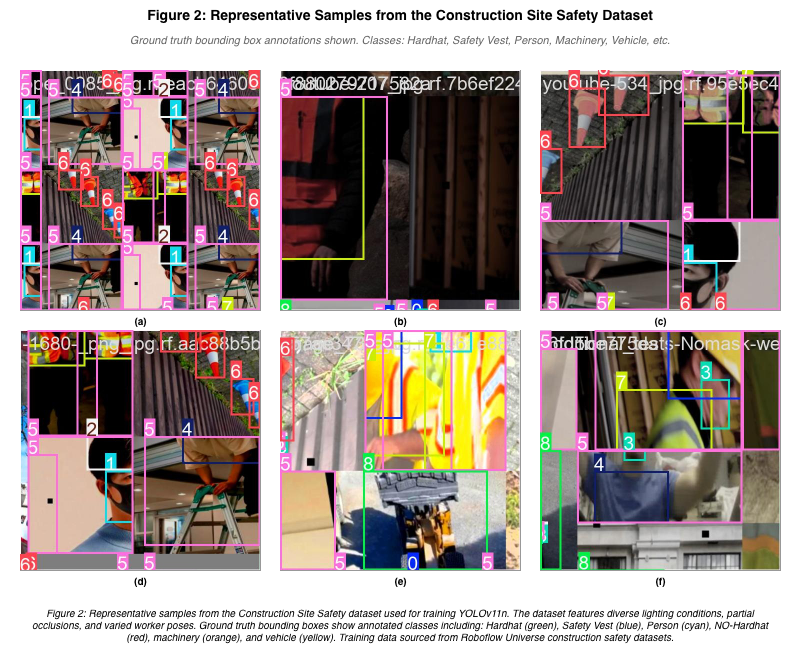
\includegraphics[width=\linewidth]{figure4.png}
    \caption{Person-Machinery Distance Analysis Over Time. Real-time Distance Measurements with Safety Zones.}
    \label{fig:distance_analysis}
\end{figure}

[cite_start]A temporal plot of this logged data, Figure \ref{fig:distance_analysis}, clearly visualizes the system's effectiveness in identifying potentially hazardous situations[cite: 146]. [cite_start]The analysis revealed several instances where the separation distance fell below predefined safety thresholds, causing the system to correctly flag these events as entries into "Caution" and "Danger" zones[cite: 147]. [cite_start]This result confirms that the framework can reliably detect proximity breaches in real time[cite: 148]. [cite_start]The generated CSV logs serve as a persistent and actionable data source, suitable not only for post-incident analysis but also for integration with automated systems to trigger immediate, on-site alerts[cite: 149].

\section{Discussion}
[cite_start]The results presented in this study validate the core hypothesis that a synergistic fusion of real-time object detection and monocular depth estimation can create a cost-effective and powerful safety monitoring tool for hazardous environments like construction sites[cite: 151]. [cite_start]Our framework successfully demonstrates the ability to move beyond generic depth maps and provide object-specific, actionable spatial data from a single 2D camera, offering a practical alternative to expensive LiDAR systems[cite: 152].

[cite_start]The system's performance, achieving an average processing speed of 25.4 FPS with a latency of 39.3 ms on Apple Silicon hardware, confirms its suitability for real-time applications where immediate feedback is paramount for accident prevention[cite: 153]. [cite_start]This real-time capability is a direct result of the multi-threaded, parallel processing architecture that executes the YOLOv11 and RT-MonoDepth models concurrently, a design choice that effectively mitigates computational bottlenecks[cite: 154].

[cite_start]The efficacy of the framework hinges on two key components: the accuracy of its perception and the reliability of its measurements[cite: 155]. [cite_start]The custom-trained YOLOv11 model exhibited high classification accuracies, notably 95\% for machinery and 91\% for safety cones, indicating its robustness in identifying critical assets within a complex construction scene[cite: 156]. [cite_start]While the 74\% accuracy for vehicles is lower, the implementation of a post-processing heuristic to reclassify vehicles based on geometric properties enhances the system's contextual understanding, which is crucial for safety analysis[cite: 157].

[cite_start]Furthermore, the automatic geometric calibration method proved to be a reliable and innovative solution to the inherent scale ambiguity of monocular depth estimation[cite: 158]. [cite_start]By leveraging a common and consistently present object on construction sites—a person—as an anthropometric reference of a known average height, the system can dynamically convert relative disparity values into absolute metric distances without requiring manual setup or pre-calibrated stereo rigs[cite: 159]. [cite_start]The successful generation of quantitative, time-series logs that correctly identified proximity breaches into "Caution" and "Danger" zones provides compelling evidence of the system's practical utility as a proactive safety monitoring tool[cite: 160].

[cite_start]Despite these promising results, several limitations and avenues for future work must be acknowledged[cite: 161]. [cite_start]The system's performance was validated on Apple Silicon hardware, and its efficiency on more resource-constrained embedded platforms like the NVIDIA Jetson series—which are more likely to be deployed in the field—remains to be empirically verified due to procurement challenges[cite: 162]. [cite_start]Additionally, the auto-calibration mechanism is dependent on the presence of a "person" in the camera's field of view and assumes a static average height of 1.7 meters[cite: 163]. [cite_start]The system's reliability could be compromised in scenarios where no personnel are visible, or when personnel height deviates significantly from the average[cite: 164]. [cite_start]Future iterations could explore more robust calibration techniques, such as using multiple object classes for reference or incorporating self-supervised scale recovery methods that do not rely on specific object detection[cite: 165]. [cite_start]Finally, while the current object taxonomy is tailored for construction sites, its performance under adverse environmental conditions such as poor lighting, fog, or heavy dust has not yet been assessed[cite: 166]. [cite_start]Future research should focus on stress-testing the framework's robustness in these challenging but realistic scenarios to ensure its reliability for all-weather, round-the-clock deployment[cite: 167].

\section{Conclusions}
[cite_start]This research successfully developed and validated a novel, cost-effective deep learning framework for real-time proximity monitoring on construction sites, addressing the critical need for affordable advanced safety systems[cite: 169]. [cite_start]By integrating a YOLOv11 object detection model with an RT-MonoDepth monocular depth estimation network in a parallelized processing pipeline, our system provides precise, object-specific metric distance information from standard 2D video streams[cite: 170]. The framework demonstrated robust real-time performance, achieving processing speeds capable of immediate hazard detection in dynamic environments, a critical factor for deployment on embedded systems as highlighted by Cheng Feng et al. (2024) [cite_start][cite: 171].

[cite_start]The key contribution of this work lies in its synergistic approach, fusing state-of-the-art perception models, such as the highly effective YOLOv11 for intelligent recognition at construction sites (He et al., 2024; Jocher et al., 2023), into a unified, deployable tool that is more powerful than its individual components[cite: 173]. [cite_start]The implementation of an automatic geometric calibration function using detected personnel as an anthropometric reference proved to be an effective method for resolving scale ambiguity, a known challenge in monocular depth estimation (Masoumian et al., 2022)[cite: 174]. [cite_start]This approach enables accurate 3D reconstruction and Euclidean distance calculations, building upon recent advancements in self-supervised monocular depth estimation and scale recovery for construction scene analysis (Shen et al., 2023) and indoor environments (Ji et al., 2021)[cite: 175]. [cite_start]Empirical validation through quantitative logging confirmed the system's ability to reliably detect and flag proximity breaches against predefined safety zones[cite: 176]. [cite_start]This research pioneers a practical, vision-based safety solution that significantly lowers the barrier to entry for advanced situational awareness technology, presenting a viable path toward reducing the high rate of fatalities and injuries that plague the construction industry[cite: 177].

\begin{thebibliography}{99}
\bibitem{feng2024realtime}
Feng, C. et al. (2024, October 27). Real-Time monocular depth estimation on embedded systems. \textit{IEEE Conference Publication | IEEE Xplore}.

\bibitem{feng2024yolo}
Feng, R., Miao, Y., \& Zheng, J. (2024, December 1). A YOLO-Based intelligent Detection algorithm for risk Assess-Ment of construction sites. \textit{TUP Journals \& Magazine | IEEE Xplore}.

\bibitem{he2024research}
He, L., Zhou, Y., Liu, L., \& Ma, J. (2024). Research and application of YOLOV11-Based object segmentation in intelligent recognition at construction sites. \textit{Buildings}, 14(12), 3777.

\bibitem{jocher2023ultralytics}
Jocher, G., Qiu, J., \& Chaurasia, A. (2023). Ultralytics YOLO (Version 8.0.0) [Computer software].

\bibitem{ji2021monoindoor}
Ji, P., Li, R., Bhanu, B., \& Xu, Y. (2021). MonoIndoor: Towards good practice of self-supervised monocular depth estimation for indoor environments. In \textit{Proceedings of the IEEE/CVF International Conference on Computer Vision} (pp. 12787-12796).

\bibitem{masoumian2022monocular}
Masoumian, A., Rashwan, H. A., Cristiano, J., Asif, M. S., \& Puig, D. (2022). Monocular Depth Estimation Using Deep Learning: A Review. \textit{Sensors}, 22(14), 5353.

\bibitem{pan2021roles}
Pan, Y., \& Zhang, L. (2021). Roles of artificial intelligence in construction engineering and management: A critical review and future trends. \textit{Automation in Construction}, 122, 103517.

\bibitem{shen2023selfsupervised}
Shen, J., Yan, W., Qin, S., \& Zheng, X. (2023). A self-supervised monocular depth estimation model with scale recovery and transfer learning for construction scene analysis. \textit{Computer-Aided Civil and Infrastructure Engineering}, 38(9), 1142–1161.

\bibitem{yu2021yolo}
Yu, J., \& Choi, H. (2021). YOLO MDE: Object Detection with Monocular Depth Estimation. \textit{Electronics}, 11(1), 76.

\bibitem{zhang2025review}
Zhang, Z., Zhang, Y., Li, Y., \& Wu, L. (2025). Review of monocular depth estimation methods. \textit{Journal of Electronic Imaging}, 34(2), 020901.

\end{thebibliography}